%%%%%%%%%%%%%%%%%%%%%%%%%%%%%%%%%%%%%%%%

\begin{edXchapter}{Trigonometry}
\begin{edXsection}{Radian}
\begin{edXvertical}
%%%%%%%%%%%%%%%%%%%%%%%%%%%%%%%%%%%%%%%

%---- Question 1 -------------------------------------------------------%

%---- Problem--------------------------%
\begin{edXproblem}{ Radian to Degree conversion }
다음 표의 빈 칸에 알맞은 값을 써 넣어라.\\ 
(TODO: Use Drag and Drop method) \\


%--- Answer Box-----------------------%
%\edXabox{expect="16" type="numerical"}

%--- Solution -----------------------%
\begin{edXsolution}

\end{edXsolution}

\end{edXproblem}
%-----End of Question 1--------------------------------------------------------%

%---- Question 2 ----------------------------------------------------------%

%--- Problem ------------------------%
\begin{edXproblem}{ Circular sector's length of an arc and area }
다음 부채꼴들의 호의 길이와 넓이를 구하여라.
(TODO: Add answer Box)

\begin{itemize}

\item
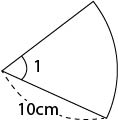
\includegraphics[width=0.2\textwidth]{p2-1}\\ 
\item
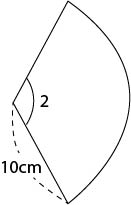
\includegraphics[width=0.2\textwidth]{p2-2}\\ 
\item
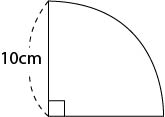
\includegraphics[width=0.25\textwidth]{p2-3}\\ 

\end{itemize}

%--- Answer Box---------------------%

%--- Solution ----------------------%

\end{edXproblem}
%--- End Of Question2 -------------------------------------------------%

%%%%%%%%%%%%%%%%%%%%%%%%%%%%%%%%%%%%%%%
\end{edXvertical}
\end{edXsection}
\end{edXchapter}
%%%%%%%%%%%%%%%%%%%%%%%%%%%%%%%%%%%%%%%
